\chapter{Prototipos estructurales}\label{cap:prototipos}

% --- INTRODUCCIÓN  ---

El análisis independiente de los campos de precipitación total (Capítulo~\ref{cap:resultados_tp}) y viento a 10 metros (Capítulo~\ref{cap:resultados_wind10}) desarrollado en los capítulos anteriores reveló que ambas variables exhiben transformaciones estructurales profundas y cualitativamente distintas a lo largo del ciclo de vida ciclónico, con una reorganización espacial que depende de la intensidad dinámica del sistema.

Sin embargo, la descripción separada de cada campo no permite cuantificar la diferenciación espacial conjunta entre los campos de circulación y precipitación en un único marco de referencia. 
Para cerrar esta brecha analítica, el presente capítulo introduce una representación sintética denominada \textit{prototipo estructural acoplado}: una visualización integrada que superpone, en el mismo dominio lagrangiano, los campos de densidad de probabilidad densidad espacial (PDF) y los patrones EOF dominantes de ambas variables simultáneamente.

Cada prototipo combina cuatro capas de información geométrica: (i) los contornos PDFe de los cuartiles 75 y 90 para la precipitación (azul) y el viento (rojo), que mapean las zonas de mayor concentración probabilística de máximos; (ii) las líneas de carga positiva (sólida) y negativa (punteada) del primer modo EOF para ambas variables (verde para precipitación, naranja para viento), que identifican los patrones espaciales de mayor variabilidad; y (iii) las coordenadas modales ($\Delta x$, $\Delta y$) de cada campo respecto al centro del vórtice (0,0), representadas mediante estrellas. El dominio de análisis corresponde al marco lagrangiano de $20^{\circ} \times 20^{\circ}$ centrado en el núcleo ciclónico, delimitado por una máscara circular de radio $9{,}5^{\circ}$ que recorta el perímetro de cada panel. Se presentan dos versiones: la Población Global (Fig.~\ref{fig:prototipo_global}) y el subconjunto de ciclones de alta vorticidad p90 (Fig.~\ref{fig:prototipo_p90}), organizadas en una matriz de $3 \times 4$ paneles (regiones $\times$ fases evolutivas), facilitando la lectura comparativa de la diferenciación entre campos a lo largo de todo el ciclo de vida.

\section{Población Global}\label{sec:prototipo_global}

\begin{figure}[H]
\centering
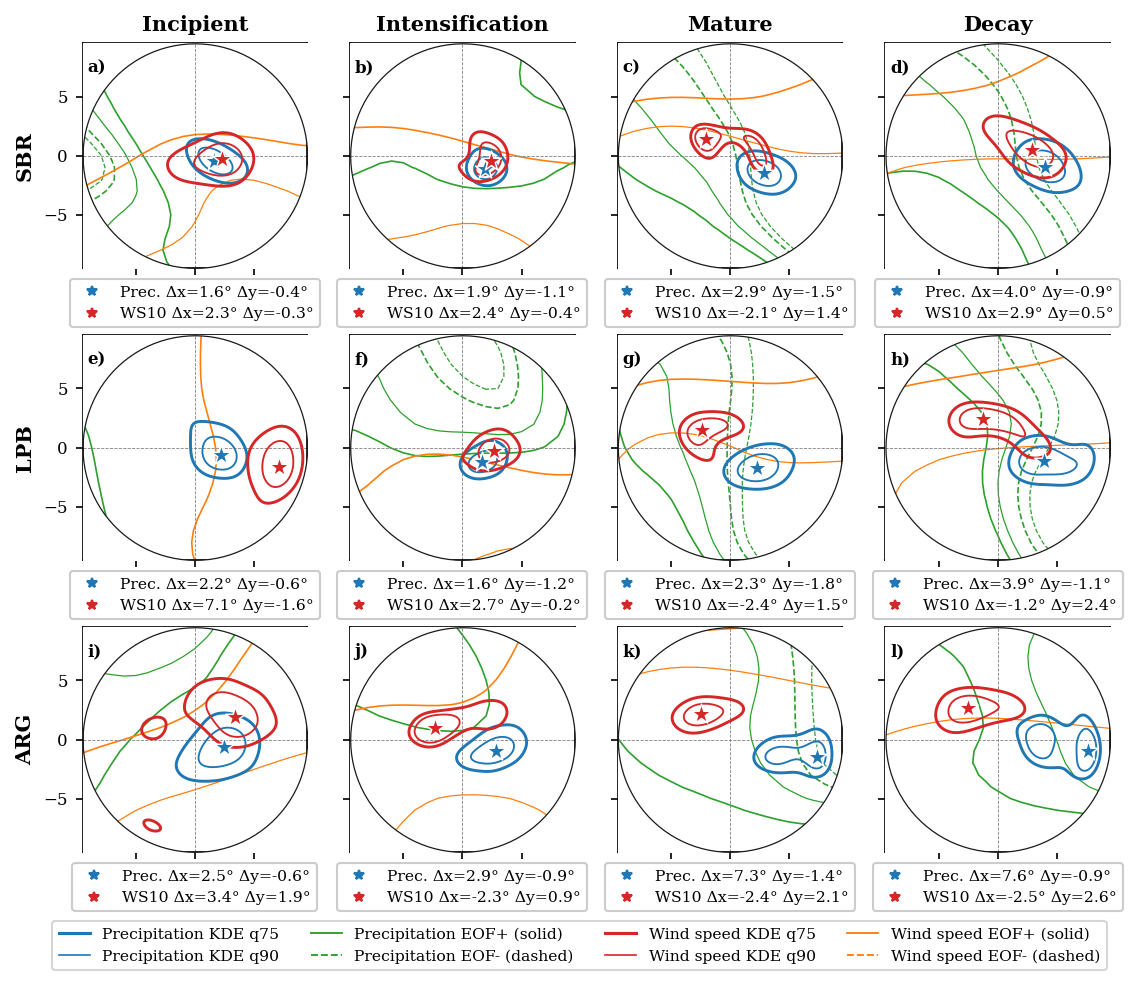
\includegraphics[width=\textwidth]{images/prototipos/prototipo_12panels_global.png}
\caption[Prototipos estructurales acoplados — Población Global]{Prototipos estructurales acoplados para la Población Global de ciclones extratropicales del Atlántico Sudoccidental. Cada panel superpone en el dominio lagrangiano $20^{\circ} \times 20^{\circ}$ centrado en el vórtice (0,0) los contornos PDFe de los cuantiles 75 y 90 de precipitación total (azul, línea gruesa y delgada respectivamente) y viento a 10 m (rojo), junto con las cargas positivas (línea sólida) y negativas (línea punteada) del EOF1 de precipitación (verde) y viento (naranja). Las estrellas azul y roja indican las coordenadas modales ($\Delta x$, $\Delta y$) de cada campo. La matriz organiza las regiones de ciclogénesis en filas (SBR, LPB, ARG) y las fases evolutivas en columnas (Incipiente, Intensificación, Madurez, Decaimiento). La máscara circular delimita el dominio a un radio de $9{,}5^{\circ}$.}
\label{fig:prototipo_global}
\end{figure}

La Figura~\ref{fig:prototipo_global} presenta los prototipos estructurales acoplados para la Población Global. Cada panel integra en un único espacio de representación la geometría probabilística de los máximos de ambas variables con los patrones de mayor variabilidad explicada (EOF1), proporcionando una lectura simultánea de la ubicación preferencial de los forzantes dinámicos de precipitación y circulación a lo largo del ciclo de vida. 

Esta figura se construyó a partir de los campos PDFe calculados sobre la grilla lagrangiana fija (Sección~\ref{subsec:kde_tp_global} para precipitación y Sección~\ref{sec:kde_espacial_global} para viento), combinados con el primer autovector espacial de los análisis EOF independientes (Sección~\ref{sec:eof_tp} y Sección~\ref{sec:eof_wind10}, respectivamente). 
Los contornos de densidad fueron suavizados mediante un filtro gaussiano ($\sigma = 2$) antes de trazar los niveles correspondientes a los cuantiles 75 y 90 de la distribución acumulada, siguiendo el criterio de región de mayor densidad (HDR). 
Su inclusión tiene como propósito sintetizar, en una visualización integrada, la coexistencia espacial o la diferenciación entre los campos de circulación y precipitación en los ciclones ordinarios, estableciendo la línea base respecto de la cual se comparará el subconjunto de alta vorticidad en la sección siguiente.

Durante las fases incipiente e intensificación (paneles a--f), los prototipos de la Población Global exhiben un patrón de co-localización relativa entre los máximos de precipitación y viento. En SBR (paneles a--b), los contornos PDFe de ambas variables se superponen parcialmente en el entorno del cuadrante oriental, con las modas de precipitación (estrella azul) y viento (estrella roja) separadas apenas $0{,}5^{\circ}$--$1^{\circ}$ en latitud, mientras que las cargas del EOF1 de viento (naranja sólida) se extienden hacia el sector noroccidental. En LPB (paneles e--f), los núcleos de densidad de precipitación se sitúan levemente al este del centro, en tanto los de viento se posicionan al suroeste durante la incipiencia, con una separación modal que oscila entre $4{,}9^{\circ}$ y $5{,}5^{\circ}$ en la dirección zonal. En ARG (paneles i--j), el patrón es bimodal desde las etapas tempranas: el PDFe de viento se concentra al suroeste del vórtice mientras el de precipitación lo hace al noreste, anticipando la divergencia estructural que se consolida en la madurez. Esta co-localización parcial durante las fases iniciales refleja que, en el régimen promedio, los forzantes frontales del WCB organizan ambos campos en el mismo sector activo del ciclón, antes de que la diferenciación interna de la estructura ciclónica imponga geometrías distintas.

Al transitar hacia la madurez (paneles c, g, k) y el decaimiento (paneles d, h, l), la arquitectura del prototipo se modifica de manera sistemática aunque moderada en la Población Global. Los contornos PDFe de viento se desplazan hacia el sector noroccidental y occidental, coherentemente con el aumento de los gradientes de presión en el flanco posterior del ciclón, mientras que los de precipitación se expanden difusamente hacia el este y sureste. Esta separación, cuantificada por la distancia entre estrellas modales, alcanza valores de hasta $5^{\circ}$--$7^{\circ}$ en la dirección zonal para SBR y LPB durante la madurez (paneles c, g), incrementándose en el decaimiento. Sin embargo, tanto los contornos PDFe como las cargas EOF1 mantienen en la Población Global una extensión espacial considerable, sin que ningún campo colapse hacia una geometría angosta y bien definida. Este comportamiento difuso refleja la heterogeneidad estructural inherente al catálogo completo, donde la integración de ciclones con distintas tasas de oclusión, profundidades de vórtice y ambientes termodinámicos diluye la señal espacial de cualquier subconjunto estructuralmente coherente.

La comparación regional revela asimetrías en la dinámica de separación. En ARG (paneles i--l), la divergencia entre los PDFe de viento y precipitación es la más pronunciada desde las fases iniciales, con la moda de viento desplazada sistemáticamente hacia el suroeste ($\Delta x < 0$, $\Delta y > 0$) en tanto la de precipitación mantiene valores positivos en ambas componentes. Este comportamiento contrasta con SBR y LPB, donde la separación meridional es menor y la distribución de precipitación es más extensa, reflejando el mayor acceso a humedad oceánica y la mayor variabilidad de trayectorias de las celdas de precipitación. Estas diferencias regionales son coherentes con los patrones individuales descritos en los capítulos anteriores y confirman que la síntesis estructural del prototipo no promedia estas diferencias sino que las preserva en la lectura integrada.

\section{Subconjunto de alta vorticidad (p90)}\label{sec:prototipo_p90}

\begin{figure}[H]
\centering
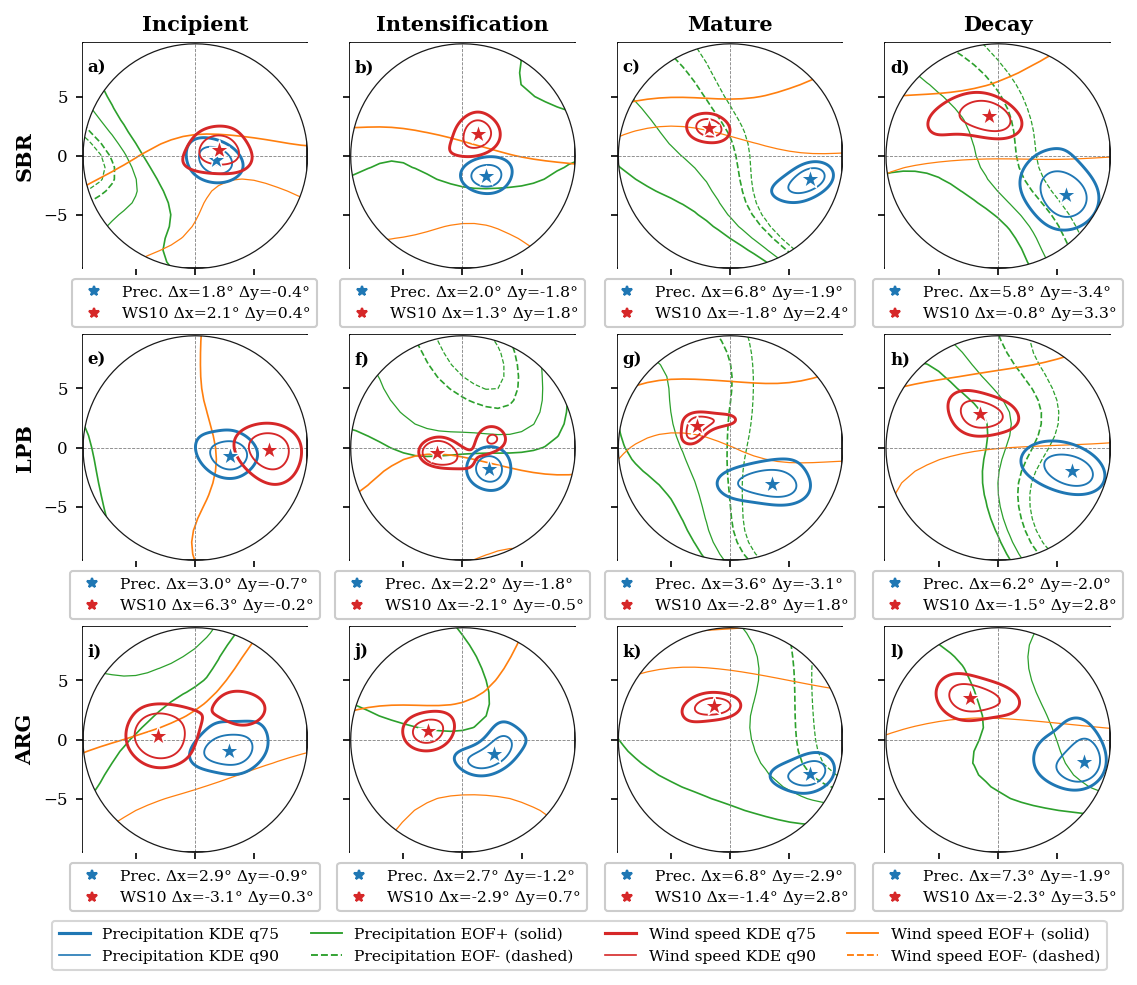
\includegraphics[width=\textwidth]{images/prototipos/prototipo_12panels_p90.png}
\caption[Prototipos estructurales acoplados — Subconjunto p90]{Prototipos estructurales acoplados para el subconjunto de ciclones de alta vorticidad (percentil 90 de vorticidad máxima). El formato de paneles, la disposición matricial ($3 \times 4$, regiones $\times$ fases), la simbología de colores y la escala del dominio lagrangiano son idénticos a los de la Figura~\ref{fig:prototipo_global}, permitiendo cuantificar directamente la transformación estructural que experimentan los sistemas de profundificación acelerada respecto a la climatología general.}
\label{fig:prototipo_p90}
\end{figure}

La Figura~\ref{fig:prototipo_p90} presenta los prototipos estructurales acoplados para el subconjunto de ciclones de alta vorticidad (p90). Construida con el mismo procedimiento metodológico que la Figura~\ref{fig:prototipo_global} pero restringida al estrato de sistemas con vorticidad máxima en el percentil 90, esta visualización está incluida para cuantificar la diferenciación espacial entre los campos de circulación y precipitación en los sistemas de máxima profundificación del Atlántico Sudoccidental, cerrando el argumento analítico desarrollado a lo largo de los capítulos de precipitación y viento. La comparación directa entre ambas figuras —posible gracias a la escala, simbología y disposición matricial idénticas— permite evaluar si la intensificación dinámica amplifica o reorganiza cualitativamente la arquitectura de acoplamiento entre variables.

El contraste visual con la Población Global es inmediato y profundo. En la fase de madurez de SBR (panel c), el PDFe de precipitación (azul) colapsa hacia una estructura compacta y desplazada hacia el este-sureste ($\Delta x = 6{,}8^{\circ}$, $\Delta y = -1{,}9^{\circ}$), mientras que el PDFe de viento (rojo) se concentra en el cuadrante noroeste ($\Delta x = -1{,}8^{\circ}$, $\Delta y = 2{,}4^{\circ}$). La separación angular entre ambas modas supera los $8^{\circ}$ en distancia euclídea, en contraste con los $3^{\circ}$--$4^{\circ}$ observados en la Población Global. Este patrón de separación cruzada —precipitación al este-sureste, viento al noroeste— se reproduce con notoria consistencia en LPB (paneles g y h) y, de manera más atenuada, en ARG (paneles k y l), donde la precipitación se desplaza hacia el este ($\Delta x = 6{,}8^{\circ}$) y el viento mantiene su posición al noroeste ($\Delta x = -1{,}4^{\circ}$, $\Delta y = 2{,}8^{\circ}$). Esta firma geométrica de cuadrantes opuestos constituye la expresión cuantitativa de la diferenciación espacial entre campos en los ciclones de máxima profundificación de la región.

La génesis de esta diferenciación en los sistemas de alta vorticidad obedece a la convergencia de los procesos de oclusión severa que se documentaron en los análisis individuales de cada variable. El patrón de viento al noroeste emerge del ciclo de vida tipo Shapiro-Keyser: la cinta transportadora fría (\textit{cold conveyor belt}, CCB) se enrolla alrededor del núcleo del sistema ocluido, generando el máximo de circulación de bajo nivel en el sector posterior izquierdo del vórtice, donde el gradiente de presión entre el centro de bajas y la dorsal circundante es más pronunciado \citep{schultz2021antecedents}. Simultáneamente, la intrusión seca (\textit{dry intrusion}) penetra desde la alta troposfera hacia el núcleo central del ciclón, erradicando la convección profunda en el dominio central y generando el característico pasillo libre de precipitación (\textit{dry slot}). Como consecuencia, el remanente de humedad del WCB es arrastrado por la circulación ciclónica hacia la periferia, quedando confinado en el frente retrocedido (\textit{bent-back front}) y formando la banda de precipitación enroscada (\textit{wrap-around precipitation}) en el cuadrante sureste y sur \citep{shapiro1990life}. La superposición de estos dos procesos, que operan simultáneamente pero en cuadrantes opuestos, es precisamente lo que genera la configuración de cuadrantes diferenciados que captura el prototipo p90.

La fase de decaimiento (paneles d, h, l) consolida y exacerba esta separación para los tres regímenes regionales. En SBR (panel d), la moda de precipitación se desplaza aún más hacia el este ($\Delta x = 5{,}8^{\circ}$, $\Delta y = -3{,}4^{\circ}$) mientras el viento migra al norte ($\Delta x = -0{,}8^{\circ}$, $\Delta y = 3{,}3^{\circ}$), aumentando la separación euclídea a más de $9^{\circ}$. En LPB (panel h), los contornos PDFe de precipitación se estrechan en una banda arqueada hacia el sur-sureste, en tanto el viento mantiene su núcleo compacto al noroeste, con una separación modal de $7{,}7^{\circ}$ en latitud. Este comportamiento refleja que, a medida que el ciclón se disipa, la banda enroscada sigue orbitando el margen de la intrusión seca incluso cuando el gradiente de presión general se debilita, mientras que el núcleo de viento se sostiene por la inercia ciclónica y la advección de vorticidad remanente. Las cargas del EOF1 de viento (naranja) mantienen su orientación noroeste-suroeste en todas las regiones durante el decaimiento, mientras que las del EOF1 de precipitación (verde) adquieren una curvatura arqueada hacia el sur, coherente con la geometría de la banda periférica documentada en la Sección~\ref{subsubsec:eof1_tp_p90}.

Las diferencias regionales en el grado de separación reflejan la modulación de los forzantes de superficie sobre la dinámica de oclusión. En SBR y LPB, el acceso a los flujos de calor latente oceánico y la fuerte baroclinicidad favorecen una oclusión más rápida, con intrusiones secas que penetran profundamente hasta el núcleo del vórtice y generan la separación más drástica entre cuadrantes \citep{gozzo2013air}. La disponibilidad de humedad tropical canalizada por el chorro de capas bajas \citep{vera2002cold} sostiene la banda enroscada de precipitación con mayor intensidad, incrementando la densidad en el cuadrante sureste y ensanchando la zona de alta probabilidad en la madurez y el decaimiento. En ARG (paneles i--l), la oclusión es más lenta debido a la modulación orográfica y a la menor disponibilidad de humedad oceánica, generando una separación moderada y una banda de precipitación menos intensa y más difusa, aunque la dirección de la diferenciación —precipitación al este-noreste, viento al noroeste— se mantiene consistente con las otras regiones, revelando que la topología fundamental de la reorganización espacial es universal y que su intensidad es la variable regionalmente modulada.

La fase incipiente de los ciclones de alta vorticidad (paneles a, e, i) muestra que la diferenciación aún no está plenamente desarrollada, pero ya exhibe una tendencia diferenciada respecto a la Población Global equivalente. En SBR (panel a), la moda de viento al noroeste ($\Delta x = 2{,}1^{\circ}$, $\Delta y = 0{,}4^{\circ}$) se separa de la moda de precipitación al este ($\Delta x = 1{,}8^{\circ}$, $\Delta y = -0{,}4^{\circ}$), con los contornos PDFe aún parcialmente superpuestos pero con centros claramente diferenciados. En LPB (panel e), la separación zonal es más notable desde el inicio ($\Delta x_{\text{viento}} = 6{,}3^{\circ}$, $\Delta x_{\text{prec}} = 3{,}0^{\circ}$), reflejando que los sistemas que eventualmente alcanzarán el percentil 90 de vorticidad ya exhiben durante su génesis una asimetría frontal más pronunciada que el promedio, coherente con el mayor gradiente térmico y el mayor flujo de humedad que caracteriza a estos entornos de ciclogénesis más activos.

% SECCIÓN: DISCUSIÓN
\section{Discusión}\label{sec:discusion_prototipos}

% --- PÁRRAFO 1: Validación del enfoque lagrangiano y comparación con literatura ---

La geometría de co-localización parcial documentada en los prototipos de la Población Global durante las fases incipiente e intensificación es coherente con los resultados obtenidos por \citet{cardoso2022synoptic} para ciclones subtropicales en la región RG1 del Atlántico Sur, quienes identificaron mediante un marco lagrangiano similar —con un dominio de $20^{\circ} \times 20^{\circ}$ centrado en el vórtice— que las anomalías positivas de viento y precipitación se concentran preferentemente en el sector este y noreste del ciclón durante las etapas de desarrollo activo. No obstante, los prototipos del presente trabajo extienden este resultado de dos maneras fundamentales: primero, al incorporar explícitamente la fase evolutiva como eje de estratificación, demuestran que esta co-localización es una característica de las fases tempranas y no una propiedad estática del ciclón; segundo, al contrastar la Población Global con el subconjunto p90, evidencian que la co-localización se quiebra de manera sistemática y cuantificable precisamente en los sistemas de máxima profundificación dinámica. Esta distinción no puede inferirse de los análisis climatológicos que promedian el ciclo de vida completo \citep{gramcianinov2023impact}, y constituye el valor agregado central del enfoque de prototipos condicionales adoptado en esta tesis.

% --- PÁRRAFO 2: El desacople espacial en p90 y el modelo Shapiro-Keyser ---

La separación de cuadrantes en los prototipos p90 —viento al noroeste, precipitación al sureste y sur— representa la expresión estadística acumulada de la transición al modelo de Shapiro-Keyser documentada para el Atlántico Sur. \citet{gozzo2013air} demostraron mediante simulaciones WRF de un ciclón tipo Shapiro-Keyser en el Atlántico subtropical que los flujos de calor latente en superficie son esenciales para sustentar el desarrollo de la seclusión cálida y la intensificación del frente retrocedido, y que sin estos flujos la banda de precipitación asociada al frente retrocedido se debilita significativamente. Este resultado tiene una implicación directa para los prototipos p90: la banda de precipitación enroscada que se manifiesta en el cuadrante sureste es físicamente insostenible sin el intercambio oceánico que caracteriza a las regiones SBR y LPB. Esto explica por qué en ARG la separación entre cuadrantes es cuantitativamente menor y la banda de precipitación del prototipo p90 es más difusa: la menor disponibilidad de calor latente oceánico limita la intensidad del frente retrocedido y, con ello, la concentración de la precipitación enroscada en la periferia del vórtice. La convergencia entre las conclusiones de los experimentos de sensibilidad de \citet{gozzo2013air} y la geometría estadística capturada por los prototipos valida que la separación de cuadrantes observada no es un artefacto del proceso de promediado, sino la huella sistemática de un mecanismo dinámico bien caracterizado.

% --- PÁRRAFO 3: Comparación con estudios del Hemisferio Norte y transferibilidad del marco conceptual ---

La arquitectura de cuadrantes documentada en los prototipos p90 del Hemisferio Sur guarda una correspondencia topológica directa, aunque especular, con la encontrada en ciclones explosivos del Hemisferio Norte. \citet{priestley2022improved} realizaron compositos de los sistemas en el tope del 10\% de vorticidad ciclónica en ERA5 aplicando la misma metodología de centrado lagrangiano y el mismo criterio de percentil que el presente trabajo, encontrando que los máximos de viento se concentran en el cuadrante suroeste del vórtice (equivalente al noroeste en el Hemisferio Sur por inversión de la circulación ciclónica), mientras que la precipitación organizada por el WCB se extiende hacia el noreste y sureste. 

La correspondencia geométrica entre el prototipo p90 de SBR y LPB en el Atlántico Sur y los compositos de \citet{priestley2022improved} en el Atlántico Norte es notable en términos de la distancia euclídea entre las modas de ambas variables y el grado de contracción de los contornos PDFe.

Las diferencias observadas —particularmente la mayor difusión de los contornos en el sector sur y la asimetría meridional más pronunciada en SBR— son consistentes con la mayor disponibilidad de humedad subtropical en la región y con la estructura híbrida que caracteriza a muchos de los sistemas p90 del Atlántico Sur, como documentan \citet{evans2012climatology} y \citet{gozzo2014subtropical}. Esto sugiere que la diferenciación de cuadrantes es un rasgo universal de los ciclones maduros de alta vorticidad, cuya intensidad regional está modulada por las condiciones termodinámicas del entorno de génesis.

% --- PÁRRAFO 4: Los prototipos como herramienta de diagnóstico: vínculo con el marco multivariado ---

El enfoque de prototipos estructurales desarrollado en este capítulo se alinea metodológicamente con propuestas recientes que enfatizan la necesidad de vincular explícitamente la evolución dinámica del sistema con sus manifestaciones estructurales. \citet{han2025system} proponen un marco de clasificación denominado \textit{SyCLoPS} (System Lifecycle of Precipitating Storms) para el Hemisferio Norte, diseñado específicamente para estudiar la frecuencia, estructura y contribución de precipitación y viento de cada tipo de sistema a lo largo de su ciclo de vida. Al igual que el presente trabajo, dicho marco reconoce que los ciclones extratropicales no pueden ser caracterizados por un único parámetro de intensidad y que la distribución espacial de sus campos dinámicos evoluciona de manera no lineal durante las distintas fases. La diferencia fundamental radica en que los prototipos aquí presentados no solo describen la arquitectura del sistema en términos cualitativos, sino que la cuantifican en un dominio lagrangiano estandarizado mediante la superposición de densidades de probabilidad espacial y modos dominantes de variabilidad (EOF), generando representaciones con un contenido probabilístico explícito que permite la comparación directa entre regiones. Esta combinación de geometría modal y densidad probabilística constituye, al igual que el marco propuesto por \citet{corner2025classification} mediante análisis multivariado de parámetros dinámicos, un avance hacia la caracterización objetiva y cuantificada de los sistemas de alta vorticidad en el Atlántico Sur, una región donde estudios equivalentes han permanecido hasta ahora muy limitados.

% --- PÁRRAFO 5: Limitaciones del enfoque y perspectivas futuras ---

Dos limitaciones del enfoque de prototipos merecen discusión explícita. En primer lugar, la estandarización del dominio lagrangiano en una grilla fija de $\pm 9{,}5^{\circ}$ implica que sistemas cuya banda de precipitación enroscada se extiende más allá de este radio —posible en los ciclones de mayor escala horizontal— contribuyen con densidad PDFe truncada en los bordes del dominio, subestimando la extensión real del campo de precipitación en el prototipo. Esta limitación es inherente al enfoque composito centrado y ha sido reconocida por \citet{cardoso2022synoptic}, quienes adoptaron explícitamente un dominio de $20^{\circ} \times 20^{\circ}$ precisamente para capturar los vientos extremos que pueden ocurrir hasta 500 km del centro del ciclón. En segundo lugar, la construcción de los prototipos sobre el subconjunto estático p90 de vorticidad máxima implica que la muestra incluye sistemas en distintas fases de su ciclo de vida al momento de ser catalogados, aunque la estratificación por fases mediante el algoritmo \textit{CycloPhaser} \citep{deSouza2025CycloPhaser} mitiga en gran medida este efecto al garantizar que cada instante analizado pertenece a la fase correcta del ciclón individual. Estas limitaciones abren líneas de trabajo futuro: la extensión del dominio a $30^{\circ} \times 30^{\circ}$ para ciclones de gran escala, y la estratificación adicional por velocidad de traslación del sistema —un factor que, como señalan \citet{gramcianinov2023impact}, modula directamente la duración del forzante y la extensión espacial de los campos dinámicos— permitirían refinar los prototipos hacia representaciones más completas de la diversidad estructural de los ciclones de alta vorticidad del Atlántico Sur.

\section{Síntesis}\label{sec:sintesis_prototipos}

Los prototipos estructurales acoplados sintetizan, en una representación geométrica única, la evolución diferencial de la organización espacial de los campos de precipitación y viento asociada a los ciclones extratropicales del Atlántico Sudoccidental a lo largo de su ciclo de vida. En la Población Global, los campos de precipitación y viento exhiben durante las fases incipiente e intensificación una co-localización relativa en el cuadrante oriental, con separaciones modales moderadas que reflejan la organización frontal del WCB como forzante común. A medida que los sistemas evolucionan hacia la madurez y el decaimiento, los campos se separan gradualmente manteniendo geometrías difusas que reflejan la heterogeneidad estructural del catálogo general.

En contraste, el prototipo p90 revela una reorganización cualitativa que emerge de la oclusión severa. La superposición simultánea de los PDFe y EOF1 de ambas variables en el mismo dominio cuantifica la diferenciación espacial en su expresión más nítida: los sistemas de alta vorticidad maduros y en decaimiento presentan los máximos de viento concentrados en el cuadrante noroeste, dominado por la cinta transportadora fría y la circulación del vórtice ocluido, mientras que los máximos de precipitación quedan relegados al cuadrante sureste y sur, confinados en la banda enroscada que orbita el margen de la intrusión seca. Esta configuración de campos en cuadrantes diferenciados, con separaciones que superan los $8^{\circ}$--$9^{\circ}$ en la madurez y el decaimiento de SBR y LPB, constituye la firma diagnóstica de la estructura ocluida en esta región y no tiene equivalente en la Población Global.

Desde el punto de vista de la dinámica sinóptica, este hallazgo implica que los sistemas de alta vorticidad del Atlántico Sur no pueden ser caracterizados mediante la co-ubicación simplificada de sus campos de precipitación y circulación.
El centro de máxima variabilidad de precipitación y el centro de máxima variabilidad de viento operan en cuadrantes geográficamente opuestos respecto al centro del vórtice, con un desfase espacial que se incrementa a medida que el sistema alcanza su máxima profundidad dinámica.
En conclusión, los prototipos presentados en este capítulo constituyen la síntesis espacial definitiva de los modos de covarianza (MEOF) identificados en el Capítulo~\ref{chap:meof}. Esta asimetría estructural refleja la reorganización física del vórtice durante la oclusión, donde la intrusión seca desplaza la convección hacia la periferia mientras la cinta transportadora fría consolida la circulación de bajo nivel en el sector posterior, validando cuantitativamente que la separación de cuadrantes es la huella sistemática y predecible de la arquitectura dinámica del ciclón maduro.
